\chapter{Lec 24 - Basics of computer vision}

\section{Image representation}
An \textbf{image} is a spatial distribution (two- or three-dimensional) of a physical entity that contains information related to the object (scene) that the image represents. That distribution can be represented as a continuous function that associates, to each point in the plane/space, the intensity of the physical entity at that point $f : \mathbb{R}^{2} \rightarrow \mathbb{R}$(or $f : \mathbb{R}^{3} \rightarrow \mathbb{R}$ for three-dimensional images).\newline
\textbf{Example:}\newline
Let's consider a monochrome image expressible by a continuous function with two independent variables:
\[f(n,m), f: \mathbb{R} \times \mathbb{R} \rightarrow \mathbb{R}\]
\begin{itemize}
    \item \textit{n, m} are the independent spatial coordinates of the image plane
    \item $f(n,m)$ gives the intensities of the measured physical quantity (usually light) at position ($n,m$).
\end{itemize}

\subsection{Digitization}
For digital processing is required a discrete representation of the images. This discretization process is composed by:
\begin{itemize}
    \item \textbf{sampling:} can be expressed as a partition of the image plane in a grid of cells.
    \item \textbf{quantisation:} conversion from the continuous range of values of image intensity to a discrete and finite set of grey values [0-255].
\end{itemize}
\subsection{Digital image representation}
Images can be seen as a Cartesian coordinates system.
\[
    f[n,m] = 
    \begin{bmatrix}
    \ddots & \vdots & \vdots& \vdots & \\
    \dots & f[-1,1] & f[0,1] & f[1,1] & \dots\\
    \dots & f[-1,0] & f[0,0] & f[1,0] & \dots\\
    \dots & f[-1,-1] & f[0,-1] & f[1,-1] &\dots\\
     & \vdots & \vdots & \vdots & \ddots\\
    \end{bmatrix}
\]
where $f[n,m]$ is a \textbf{discrete} function and $n,m$ correspond to rows and columns of a matrix. Each element of the matrix is a \textbf{pixel} and each pixel can have a value, in case of  a grey scale image, between 0-255. By convention, $f[0,0]$ is the center of the image.

\section{Colors}
\subsection{RGB representation}
\begin{center}
    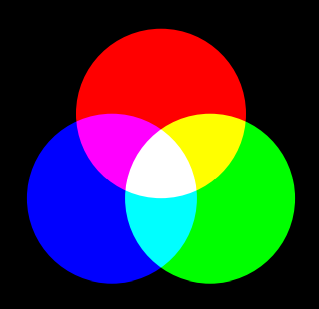
\includegraphics{images/RGB.png}
\end{center}
In the RGB (Red, Green, Blue) system, the primary colors are:
\begin{itemize}
    \item red
    \item green
    \item blue
\end{itemize}
By composing two primary colors, you obtain secondary colors:
\begin{itemize}
    \item cyan = green + blue
    \item magenta = red + blue
    \item yellow = red + green
\end{itemize}
By composing all the primary colors, you obtain white.\newline
An RGB-encoded image consists of three channels, one for each component, where each color is obtained mixing red, green and blue values. If you use 8 bit to represent each component, the number of distinct colors that can be represented in the image is $(2^{8})^{3} = 16 777 219$.\newline
The function that describes an RGB-image is the following:
$$f[n,m] = \left[
\begin{array}{c}
r[n,m]\\
g[n,m]\\
b[n,m]
\end{array}\right]
$$

\subsection{HSV representation}
\begin{center}
    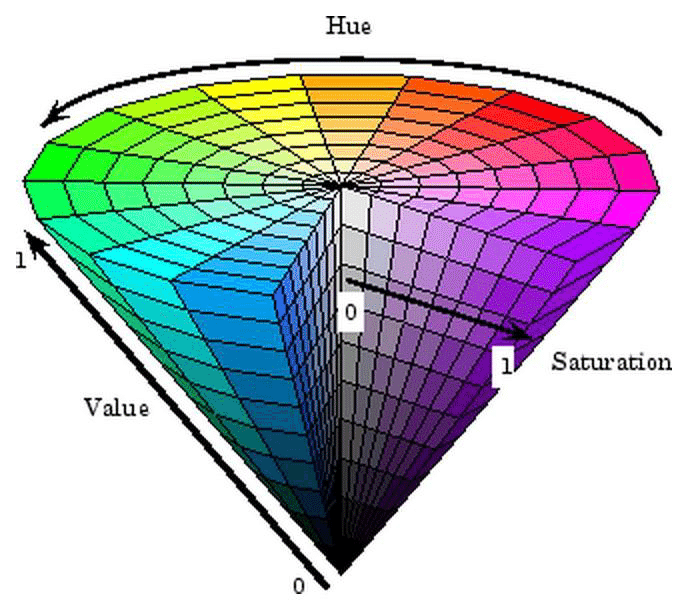
\includegraphics[scale = 0.3]{images/HSV.png}
\end{center}
The HSV representation specifies colors in term of:
\begin{itemize}
    \item \textbf{hue:} dominant color
    \item \textbf{saturation:} it measures how far you are from the fully saturated color (in which you don't have any grey).
    \item \textbf{lightness:} color brightness. While saturation measures the “dilution” of hue with white, brightness indicates dilution with black.
\end{itemize}
HSV representation is closer to how people perceive colors.

\section{Filters}
\textbf{Filtering:} Forming a new image whose pixel values are transformed from the original ones.\newline
The goals of filtering are:
\begin{itemize}
    \item \textbf{extract} useful information
    \item \textbf{transform} images into another domain where we can modify/enhance image properties.
\end{itemize}
\subsection{Linear Filters}
We define a filter as a unit that converts an input function $f[n,m]$ into an output function $g[n,m]$, where ($n,m$) are the independent variables. \newline
Linear filters work by moving a sliding window (kernel) through the image, pixel by pixel. The window contains coefficients which characterize the transformation. At each position, the result of the filter is calculated by combining the values of the image subtended to the window with the coefficients of the window itself. In order to compute the new value of the central pixel, the coefficients are:
\begin{itemize}
    \item multiplied by the values of the original image subtended to the window
    \item added
\end{itemize}
These filters are defined by the following mathematical operator called \textbf{convolution}:
\[(f * h)[n,m] = \sum_{k,l}f[k,l]h[n-k, m-l]\]
where $h$ is the \textit{kernel}.\newline \newline
\textbf{Borders:}\newline
Given an $n \times n$ kernel, its external row/column coincides with the border of the image when the center of this mask is at distance $\frac{n-1}{2}$ from the edge. If you move further out, part of the window \textit{leaves} the image.\newline
This situation can be managed in three different ways:
\begin{itemize}
    \item limit the movement of the mask, keeping it at a minimum distance of $\frac{n-1}{2}$ from the edges.
    \item duplicate the external rows/columns of the image
    \item enlarge the image with rows/columns of zeros
\end{itemize}
Solution 1 gives reliable results, but produces a different size image from the original. Solutions 2 and 3, on the other hand, give results that are not exactly authentic near the edges, but are often convenient because they allow you to obtain an output image with the same size as the input one.

\subsection{Smoothing filters}
Smoothing filters are low-pass filters: they emphasize low frequencies and attenuate the high frequencies. They cause image blur, which is helpful to:
\begin{itemize}
    \item remove small details
    \item reduce noise in the image
\end{itemize}
\textbf{Examples:}
\begin{itemize}
    \item \textbf{Moving average filter} (\textit{box filter}) in which all the kernel coefficients are equal to 1.
    \begin{center}
        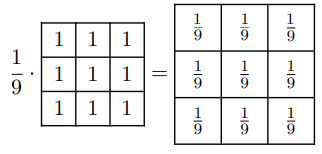
\includegraphics[]{images/box filter.png}
    \end{center}
    It is defined by the following formula:
    \[g[n,m] = \frac{1}{9}\sum_{k=-1}^{1}\sum_{l=-1}^{1}f[n-k, m-l]\]
    Basically, it replaces each pixel with an average of its neighbors. This filter can be applied in order to remove small details, to obtain blurring effect (more evident as the size of the window increases) but it is not useful to remove the so called \textit{salt and pepper noise}, because corrupted pixels affect the computation of the average, so the noise points can even tend to dilate.

\end{itemize}

\subsection{Sharpening filters}
A sharpening filter emphasizes image details. They are high pass filters that emphasize high frequencies, and penalize low frequencies.\newline
The sharpening effect is obtained in two steps:
\begin{itemize}
    \item Apply an operator that extracts the details of the image (produces an image with light values in the transition areas and dark values in the uniform areas)
    \item This result is added to the original image
\end{itemize}
One way to obtain the details is by applying a smoothing filter to an image and computing a pixel by pixel difference between the original image and the smoothed one. Then you add the resulting image to the original one to obtain the sharpening effect.
\begin{flushleft}
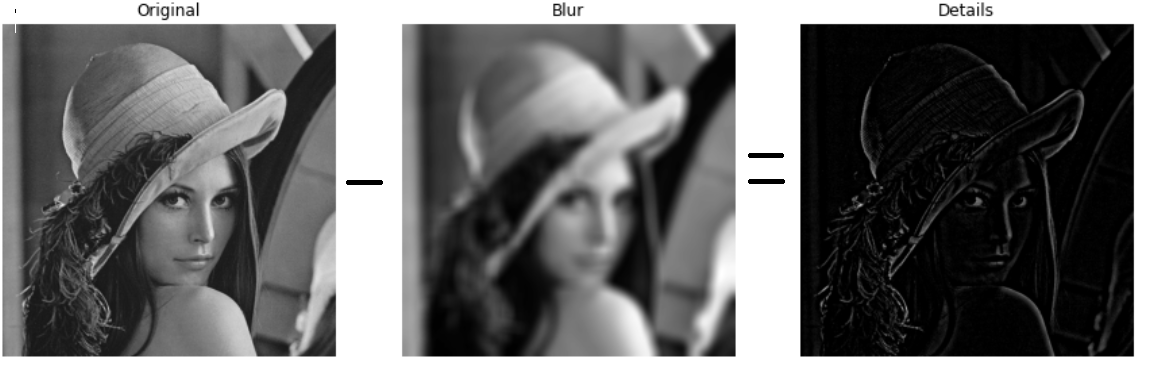
\includegraphics[scale=0.6]{images/details.png}
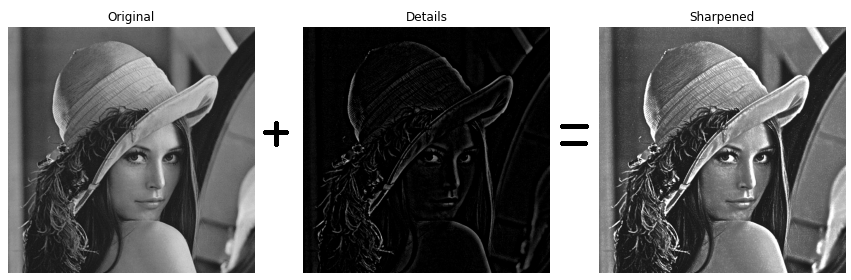
\includegraphics[scale = 0.8]{images/Lena sharpened.png}
\end{flushleft}

\section{Edge detection}
An edge is a set of connected pixels between two regions in which there is a sudden change in intensity. These discontinuities can be caused by:
\begin{itemize}
    \item Illumination discontinuity: cast shadows
    \item Change in surface orientation: shape
    \item Depth discontinuity: object boundary
    \item Surface color discontinuity
\end{itemize}
The goal of edge detection is to detect easily and automatically these regions.\newline
Basically, a simple edge detection algorithm computes the first order derivative of the intensity function of an image and detects as edges the extremes of the derivative function.
\begin{flushleft}
    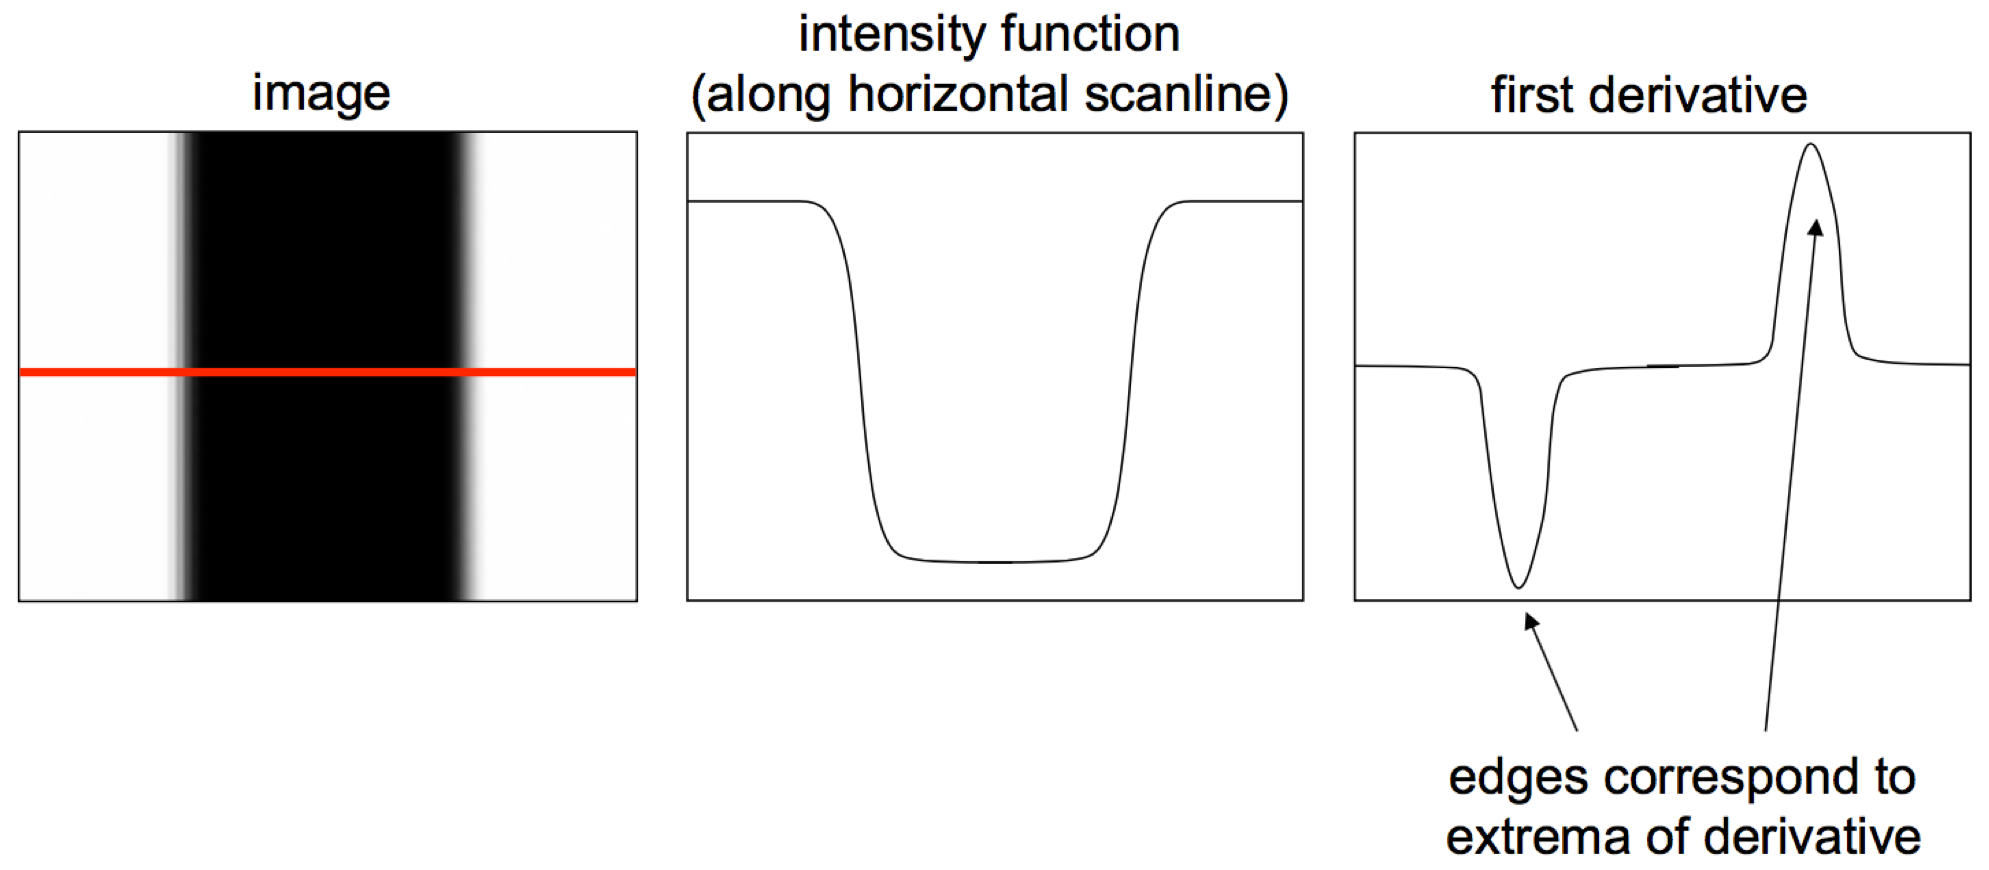
\includegraphics[scale = 0.4]{images/edge detection.png}
\end{flushleft}

\subsection{Discrete approximation of the derivatives}
In order to apply a derivative operator in a digital environment, we need a discrete approximation of derivatives. 
\begin{itemize}
    \item Derivative in 1D:
    \[\frac{df}{dx} = lim_{\Delta x \rightarrow 0} \frac{f(x) - f(x - \Delta x)}{\Delta x} = f^{'}(x)\]
    \item Discrete derivative in 1D:
    \[\frac{df}{dx} = lim_{\Delta x \rightarrow 0} \frac{f(x) - f(x - \Delta x)}{\Delta x} = f^{'}(x)\]
    \[= \frac{f(x) - f(x - 1)}{1} = f^{'}(x)\]
    \[= f(x) - f(x - 1) = f^{'}(x)\]
\end{itemize}
Operators based on the first order derivative must satisfy the following properties:
\begin{itemize}
    \item have zero value in the homogeneous sections of the image (no response in constant regions)
    \item have a non-zero value along the transition areas.
\end{itemize}
Formulations satisfying these properties can be defined in terms of differences between pixel values.\\\\
According to this, a 2D derivative filter could be defined by the following kernels (central derivative):
\begin{figure}[h]
        \centering
        \begin{minipage}{0.45\linewidth}
        \centering
        \begin{tikzpicture}
            \matrix[matrix of nodes ,nodes={minimum size=0.5cm, draw}, row sep=-\pgflinewidth, column sep=-\pgflinewidth](sobel_hz){%
            1 & 1 & 1\\
            0 & 0 & 0\\
            -1 & -1 & -1\\
            };
        \end{tikzpicture}
        \caption*{Detects horizontal edges}
        \end{minipage}
        \hspace{20pt}
        \begin{minipage}{0.45\linewidth}
        \centering
        \begin{tikzpicture}
            \matrix[matrix of nodes ,nodes={minimum size=0.5cm, draw}, row sep=-\pgflinewidth, column sep=-\pgflinewidth](sobel_v){%
            1 & 0 & -1\\
            1 & 0 & -1\\
            1 & 0 & -1\\
            };
        \end{tikzpicture} 
        \caption*{Detects vertical edges}
        \end{minipage}
\end{figure}

\subsection{Image gradient}
The operators based on the first order derivative are formulated starting from \textbf{gradient}. Given a function $f(x,y)$ (2D image), the gradient vector is defined as follows:
\[
    \nabla f = 
    \begin{bmatrix}
        G_{x}\\
        G_{y}\\
    \end{bmatrix}
    =
    \begin{bmatrix}
        \frac{\partial f}{\partial x}\\
        \vspace{1pt}\\
        \frac{\partial f}{\partial y}\\
    \end{bmatrix}
\]
The image gradient is obtained by applying two-dimensional derivative filters and it provides the following information:
\begin{itemize}
    \item The partial derivatives with respect to both horizontal and vertical directions.
    \item The gradient magnitude, which indicates the intensity of the discontinuity.
    \[|| \nabla f || = \sqrt{G_{x}^{2} + G_{y}^{2}}\]
    \item The gradient direction, given by:
    \[ \theta = tan^{-1} \left (\frac{G_{y}}{G_{x}} \right)\]
    \item It points in the direction of most rapid increase in intensity.
\end{itemize}

\section{Key-points}
Edge detection is useful to extract information, recognize objects, recover geometry and viewpoint, but edges are not very robust against a number of transformations. So, it's not a good idea to use them, for example, for object detection.\newline\newline
Edges are an example of \textbf{key-point}. A key-point is a region of the image in which you have specific properties.
\begin{itemize}
    \item \textbf{flat region:} no change in all direction.
    \item \textbf{edge:} no change along the edge direction.
    \item \textbf{corner:} significant change in all directions.
\end{itemize}
Corners are \textbf{local features} that are more informative and more robust to different image transformations than edges.\\\\
\textbf{Scale invariant detection goal:} given different images of the same scene with large scale differences between them, find the same key-points independently in each image.

\section{SIFT algorithm}
SIFT is a scale invariant feature detection algorithm that applies $DoG$ both in space and over different scales. Thanks to this, it is computationally more efficient than the Harris-Laplacian algorithm. Following are the major stages of computation used to generate the set of image features:
\begin{enumerate}
    \item \textbf{Scale-space extrema detection:} The first stage of computation searches for local features over all scales and image locations using a difference of Gaussian function.
    \item \textbf{Key-point localization:} At each candidate location, a detailed model is fit to determine location and scale. Key-points are selected based on measures of their stability (\textbf{It was not covered in class}).
    \item \textbf{Orientation assignment:} One or more orientations are assigned to each key-point location based on local image gradient directions.
    \item \textbf{Key-point descriptor:} Describing the key-points as a high dimensional vector such that it is highly distinctive and invariant as possible to variations such as changes in viewpoint, illumination, translation, rotation and scale.
\end{enumerate}
\begin{center}
    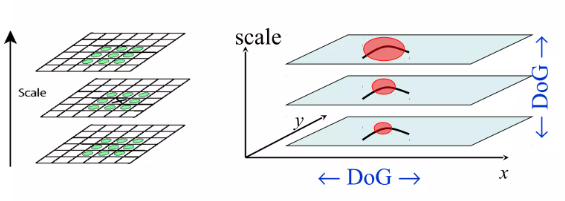
\includegraphics[]{images/DoG space scales.png}
\end{center}

\section{Bag of Visual Words}
In order to implement image classification, we need two major components:
\begin{itemize}
    \item A way to describe images. Not just local features descriptors, but a \textbf{global} representation of the image.
    \item A procedure to \textbf{compare} different images and learn a statistical model of a specific class. 
\end{itemize}
Bag Of Visual Words is a technique to describe images. The approach has its origin in text retrieval and it is an extension of the Bag of Words algorithm. In Bag Of Words, we scan through the entire document and keep a count of each word appearing in the document. Then, we create a histogram of frequencies of words and use it to describe the text document. In Bag Of Visual Words, our input are images and we use \textbf{visual words} to describe them.
\newline\newline
The pipeline follows these steps:
\begin{enumerate}
    \item Extract local features (e.g. using SIFT) from training images.
    \item Quantize the feature space (build a visual dictionary or codebook). Make this operation via clustering algorithms such as K-means. The center points, that we get from the clustering algorithm, are our visual words.
    \item For each feature of each training image, find the closest visual word in the visual dictionary and build frequency histograms (one for each training image).
    \item Compute histograms of visual words of \textbf{test} images (following the same procedure) and predict their class using the histograms of training images (e.g. using k-NN).
\end{enumerate}

\section{Convolutional Neural Networks (CNN)}
Convolutional Neural Networks are a specialized kind of NN for processing data that has a \textbf{grid-like topology} (e.g. images). The name CNN indicates that the network employs a mathematical operation called \textbf{convolution}.\newline\newline
CNN learns different levels of abstraction of the input, e.g. for images:
\begin{itemize}
    \item in the first few hidden layers, the CNN usually detects general pattern, like edges.

    \item the deeper we go into the CNN, these learned abstractions become more specific, like textures, patterns and parts of objects.

\end{itemize}
For what concerning convolution of multi-channel images, we perform the convolution for each channel and we sum up the results.
\begin{center}
    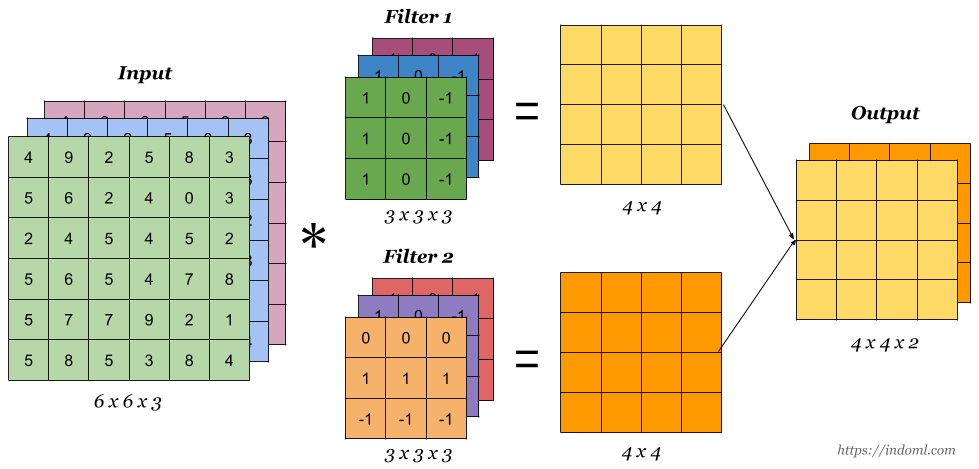
\includegraphics[scale = 0.3]{images/Convolution.png}
\end{center}

\subsection{Pooling}
Another commonly used technique in CNN is \textbf{Pooling}.\newline\newline
Pooling layer is used to reduce the size of the representations and to speed up calculations, as well as to make some features it detects a bit more robust.
\begin{itemize}
    \item \textbf{Max pooling:} It gets the maximum value of the pixels for each section of the image.

    \item \textbf{Average pooling:} It gets the average value of the pixels for each section of the image.
\end{itemize}
\begin{center}
    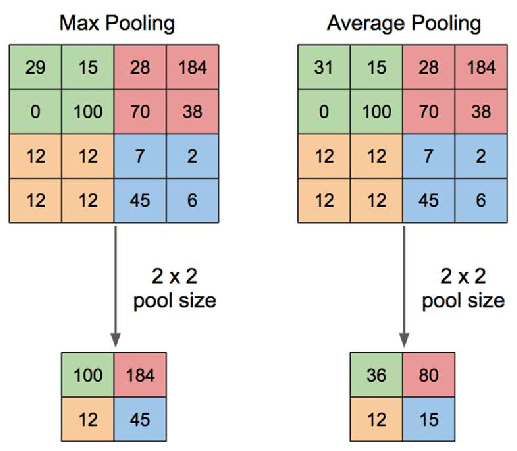
\includegraphics[scale = 0.3]{images/pooling.png}
\end{center}

\subsection{Convolution layer}
The Convolution layer applies a set of filters to the input data (performing convolution) in order to extract features or representations from the data. The result is usually passed through an activation function (ReLu) in order to achieve non linearity. \newline\newline
Basically, a CNN is a sequence of convolution layers and sub-sampling layers with a fully-connected layer at the end.
\begin{center}
    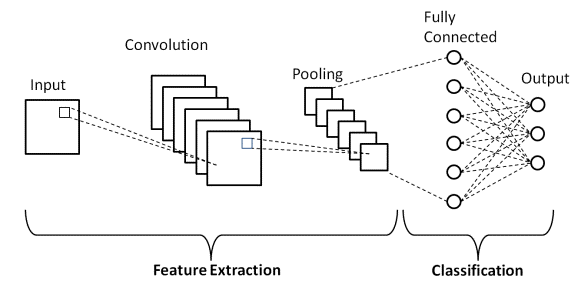
\includegraphics[scale = 0.7]{images/CNN.png}
\end{center}
